\documentclass[12pt]{extarticle}
\usepackage[utf8]{inputenc}
\usepackage[english,russian]{babel}
\usepackage{vmargin}
\usepackage{indentfirst}
\usepackage[T2A]{fontenc}
\usepackage{graphics}
\usepackage{amsthm}
\usepackage{amsbsy}
\usepackage{amsmath}
\usepackage{amssymb}
\usepackage{amsfonts}
\usepackage{mathtext}
\usepackage[pdftex,a4paper,colorlinks,linkcolor=blue,citecolor=blue]{hyperref}	

\usepackage{mathtext}
\usepackage{mathenv}
\usepackage[pdftex]{graphicx}
\usepackage{array}
\usepackage{graphicx,xcolor}
\usepackage{xcolor}
\usepackage{float}
\usepackage{longtable}

%\parindent = 30pt
%\hoffset = 0pt
%\voffset = 0pt
\oddsidemargin = 100pt
\topmargin = 18pt
%\headheight = 12pt
%\headsep = 25pt
\textheight = 700pt
\textwidth = 440pt
%\marginparsep = 10pt
%\marginparwidth = 103pt

\usepackage{tikz}
\usepackage{verbatim}

\paperwidth = 597pt
\paperheight = 845pt
\numberwithin{equation}{section}

\DeclareMathOperator{\sign}{sign}
\DeclareMathOperator{\const}{const}
\renewcommand{\Re}{\mathop{\mathrm{Re}}\nolimits}
\renewcommand{\Im}{\mathop{\mathrm{Im}}\nolimits}
\newtheorem{algorithm}{Алгоритм}[section]

\begin{document}

\begin{titlepage} \newpage 
\begin{center} МОСКОВСКИЙ ГОСУДАРСТВЕННЫЙ УНИВЕРСИТЕТ ИМ. М.В. ЛОМОНОСОВА\end{center} 
\vspace{8em} \begin{center} 
\Large Механико-математический факультет \\ \end{center}
\vspace{2em} \begin{center} 
\textsc{Отчет по практикуму на ЭВМ \linebreak 
\textbf{}} \end{center}
\vspace{6em} \newbox{\lbox} \savebox{\lbox}{\hbox{Д.Салахов}} 
\newlength{\maxl} \setlength{\maxl}{\wd\lbox} \hfill\parbox{12	cm}
{ \hspace*{10cm}\hspace*{-5cm}Студент 4 курса:\hfill\hbox to\maxl{Дамир Салахов}\\
\hspace*{10cm}\hspace*{-5cm}Преподаватель:\hfill\hbox to\maxl{Ченцова Н.Н.}}\\  \vspace{\fill}
\begin{center} Москва \\ 2018\end{center} \end{titlepage}

%\maketitle

%\renewcommand{\contentsname}{Содержание}
\tableofcontents
\renewcommand{\figurename}{График}
\renewcommand{\theequation}{\thesection.\arabic{equation}}


\newpage

\section{Постановка задачи} \label{sec:1-postanovka-zadachi}
Дано уравнение в частных производных с заданными начальными условиями:
\begin{equation}
\left\{
	\begin{aligned}
&\frac{\partial u}{\partial t} = \frac{\partial ^2 u}{\partial t^2} + u^3 - \cos \frac{\pi x}{2} \\
& x = 0: \qquad \frac{\partial u}{\partial x} = 0\\
& x = 1: \qquad u = 0 \\
	\end{aligned}
\right.
\label{eq:1-nachal-zadacha}
\end{equation}

Неизвестная функция -- $u$ от двух переменных $t$ и $x$ (переменные Эйлера), причем $$(t, x) \in Q = [0, 1] \times [0, 1].$$

Само уравнение можно перепиать в виде
\begin{equation}
\frac{\partial u}{\partial t} = \frac{\partial ^2 u}{\partial t^2} + f, \label{eq1}
\end{equation}
где $f$ -- данная функция.

Для начального момента  времени задана функция $u_0$, значения которой совпадают со значениями $u$ на отрезке $x \in [0; 1]$:
\begin{equation}
u |_{t=0} = u_0 = 0.9 \cdot (1 - x^2), \label{nu}
\end{equation}

Для решения задачи введем равномерную сетку $\omega_h$ с шагом $h$ по оси $x$ и с шагом $\tau$ по оси $t$. 
Введем константы $M$ и $N$, такие что $X = Mh$ и $T = N\tau$.

\section{Описание явной схемы схемы} \label{scheme0}
Чтобы свести дифференциальное уравнение к неявной схеме, заменим производные на разности на этом же слое сетки (за исключением производной по $t$).
Получим схему:
	\begin{align}
		&V_t= V_{x \hat x} + f,\qquad x \in \omega_h, \label{eq0-1}\\
		&V_{x, 0} = 0 \label{eq0-2}\\
		&{V^n_M} = 0 \label{eq0-3}
	\end{align}

Исходя из \ref{nu}, в качестве значений решения на нулевом слое берутся проекции на сетку $\bar{\omega}_h$ функции $u_0$, т.е.
$$V_m^0 = (u_0)_m, \qquad \mbox{где} \quad m = 0, 1, \dots M.$$

\subsection{Уравнение \ref{eq0-1}}
Распишем основные обозначения:
\begin{align*}
&V_t = \cfrac{V_m^{n+1} - V_m^n}{\tau} \label{eq0:1:1}\\
&V_{x \hat x} = \cfrac{V_{m+1}^{n} - 2V_m^{n} + V_{m-1}^{n}}{h^2} \label{eq0:1:2}
\end{align*}

Подставим \ref{eq0:1:1} и \ref{eq0:1:2} в \ref{eq0-1}, получим:
\begin{equation}
\cfrac{V_m^{n+1} - V_m^n}{\tau} = \cfrac{V_{m+1}^{n} - 2V_m^{n} + V_{m-1}^{n}}{h^2}. \label{sc}
\end{equation}

Приведем подобные и выразим $V_m^{n+1}$:
$$V_m^{n+1} = V_{m-1}^n \cdot \frac{\tau}{h^2}  + V_m^n \cdot \left( 1 - \frac{2 \tau}{h^2} \right) + V_{m+1}^n \cdot \frac{\tau}{h^2}.$$
Для ускорения дальнейших вычислений и улучшения точности введем переменную $\gamma = \tau/h$ и получим 
\begin{equation}
V_m^{n+1} = V_{m-1}^n \cdot \frac{\gamma}{h}  + V_m^n \cdot \left( 1 - \frac{2 \gamma}{h} \right) + V_{m+1}^n \cdot \frac{\gamma}{h}. \label{eq0}
\end{equation}

\subsection{Уравнения \ref{eq0-2} и \ref{eq0-3}}
Из \ref{eq0-2} следует: $$V_{1}^{n} = V_0^{n}.$$

Из \ref{eq0-3} следует, что весь последний слой сетки равен нулю: $$V_M^n = 0.$$

\subsection{Алгоритм}
Заметим, что  из \ref{eq0} $V_m^{n+1}$ для $m = 1 \dots N - 1$ на $n+1$-ом слое выражается через три точки предыдущего $n$-ого слоя (на рисунке: может заполнить любой столбец, зная его соседний столбец слева).
Для $m = M$ все также известно (они нулевые).
Уровень $m = 0$ можно вычислить, зная уровень $m = 1$.

Предзаполним в таблице первый столбец и последнюю строчку.
Далее, используя \ref{eq0} можем заполнить все оставшиеся клетки, идя сверху вниз, слева направо.
\begin{center}
\begin{tabular}{|c||c|c|c|c|c|}
\hline
$m \backslash n$ & 0 & 1 & 2 & $\cdots$ & $N$ \\
\hline
\hline
0			& $u_0 (0)$ & $V_0^1 := V_1^1$ &$V_0^2:=V_1^2$ &  $\cdots$ & $V_0^N:=V_1^N$ \\
\hline                                                 
1			& $u_0 (h)$		 & $\uparrow$ & $\uparrow$ &  &$\uparrow$ \\
\hline                                                 
2			& $u_0 (2h)$	 & $\uparrow$ & $\uparrow$ &  & $\uparrow$\\
\hline                                                 
$\vdots$ 	&  				 & $\uparrow$ & $\uparrow$ & $\ddots$ & $\uparrow$\\
\hline                                                 
$M - 1$ 	& $u_0 ((M-1)h)$ & $\uparrow$ & $\uparrow$ &  & $\uparrow$\\
\hline
$M$			& $u_0 (Mh) \equiv 0$ & $0$ & $0$ & $\cdots$  & $0$ \\
\hline
\end{tabular}
\end{center}

\subsection{Сходимость схемы} \label{sp}
Для того, чтобы понять, при каких разбиениях сходится данная схема, будем использовать спектральный признак устойчивости.

Подставим в \ref{sc} $V_m^n = \lambda^n e ^{im\varphi}$.
Тогда согласно признаку схема устойчива, если $\exists c: \quad |\lambda| < 1 + c \tau \quad \forall \varphi$.

Получим:
$$
\begin{eqnarray}
&& \cfrac{\lambda^{n+1} e^{im\varphi} - \lambda^n e ^{im\varphi}}{\tau} = \cfrac{\lambda^n e ^{i(m+1)\varphi} - 2\lambda^n e ^{im\varphi} + \lambda^n e ^{i(m-1)\varphi}}{h^2} \nonumber \\
&& \cfrac{\lambda e ^{i\varphi}- e ^{i\varphi}}{\tau} = \cfrac{e ^{2i\varphi} - 2 e ^{i\varphi} + 1}{h^2} \nonumber\\
&& \lambda - 1 = \frac{\tau}{h^2} \cdot \left( \cfrac{e ^{2i\varphi} + 1}{e ^ {i \varphi}} - 2 \right) \nonumber\\
&& \lambda = 1 + \frac{\tau}{h^2} \cdot \left( 2\cos \varphi - 2 \right) \nonumber\\
&& \lambda = 1 - \frac{4\tau}{h^2} \cdot \sin^2 \frac{\varphi}{2} \label{lam}
\end{eqnarray}
$$
Для устойчивости схемы нужно $|\lambda| \leqslant 1.$
Перепишем \ref{lam}:
$$
\begin{eqnarray}
&& \left|1 - \frac{4\tau}{h^2} \cdot \sin^2 \frac{\varphi}{2}\right| \leqslant 1\nonumber\\
&& \left|\frac{4\tau}{h^2} \cdot \sin^2 \frac{\varphi}{2}\right| \leqslant 2 \nonumber \\
&& 0 \leqslant \frac{\tau}{h^2} \cdot \sin^2 \frac{\varphi}{2} \leqslant \frac{1}{2} \nonumber
\end{eqnarray}
$$
Очевидно, что квадрат синуса больше нуля.
Так как правое неравенство должно быть верно для любых $\varphi$, то зная, что $\sin^2 \frac{\varphi}{2} \leqslant 1$, получаем необходимое условие:
\begin{equation}
\frac{\tau}{h^2}  \leqslant \frac{1}{2} \label{usl0}
\end{equation}

\section{Описание неявной схемы схемы} \label{scheme}
Для поиска численного решения задачи \ref{eq:1-nachal-zadacha} будем использовать разностную схему, в которой при аппроксимации членов используются односторонние разности:
%\begin{aligned}
%\left\{
	\begin{align}
		&V_t= \hat{V}_{x \hat x} + f,\qquad x \in \omega_h, \label{eq1-1}\\
		&\hat V_{x, 0} = 0 \label{eq1-2}\\
		&{\hat V^n_M} = 0 \label{eq1-3}
	\end{align}
%\right.
%\end{aligned}
Так же как и в предыдущей схеме \ref{scheme0} на нулевом слоне возьмем проекции на сетку:
$$V_m^0 = (u_0)_m, \qquad \mbox{где} \quad m = 0, 1, \dots M.$$

Коэффициенты перед элементами $V$ в уравнении \ref{eq1-1} задают элементы матрицы и правой части.
Таким образом с помощью этих уравнений можно получить матричное, решив которое, можно найти значения для функции $u$ на новом слое сетки.
Распишем уравнения системы для нахождения элементов матрицы.

\subsection{Уравнение \ref{eq1-1}}
Вспомним обозначения:
\begin{align}
&V_t = \cfrac{V_m^{n+1} - V_m^n}{\tau} \label{eq2:1:1}\\
&\hat V_{x \hat x} = \cfrac{V_{m+1}^{n+1} - 2V_m^{n+1} + V_{m-1}^{n+1}}{h^2} \label{eq:2:1:2}
\end{align}

Перепишем само уравнение:
$$\cfrac{V_m^{n+1} - V_m^n}{\tau} = \cfrac{V_{m+1}^{n+1} - 2V_m^{n+1} + V_{m-1}^{n+1}}{h^2} + f
$$
Приводя подобные и домножая обе части на $\tau$ и взяв $\gamma = \tau/h$
\begin{equation}
 V_{m+1}^{n+1} \cdot \cfrac{\gamma}{h} + V_m^{n+1} \cdot \left( -1 - \cfrac{2\gamma}{h}\right) + V_{m-1}^{n+1} \cdot \cfrac{\gamma}{h} = -V_m^n - f \cdot \tau
 \label{eq2:1:final}
\end{equation}

\subsection{Уравнения \ref{eq1-2} и \ref{eq1-3}}
Из уравнения \ref{eq1-2} получаем коэффициенты для нулевой строки матрицы и правой части алгебраической задачи.
\begin{align*}
&\hat V_{x, 0} = \cfrac{V_1^{n+1} - H_0^{n+1}}{h}\\
\end{align*}
Итого, домножив на $h$ получим
\begin{equation}
-V_0^{n+1} + V_{1}^{n+1} = 0 \label{eq:2final}
\end{equation}

Из уравнения \ref{eq1-3} получаем последню строку матрицы (она нулевая).

\subsection{Алгоритм}
На каждом шаге итерации сначала будем строить матрицу размера $M+1$ и правую часть для нового слоя $V^{n+1}$, используя уравнения \ref{eq2:1:final}, \ref{eq:2final}, \ref{eq1-3}.
Решив полученную систему линейное уравнение, найдем новое приближение для $u$.

Заметим, из итоговых уравнений видно, что в алгебраической задаче получились трехдиагональные матрицы.
Таким образом, полученную СЛУ можно решить методом прогонки.

\subsection{Сходимость схемы}
Действуем также, как и в \ref{sp}
Подставим в схему $V_m^n = \lambda^n e ^{im\varphi}$.
Получим:
$$
\begin{eqnarray}
&& \cfrac{\lambda^{n+1} e^{im\varphi} - \lambda^n e ^{im\varphi}}{\tau} = \cfrac{\lambda^{n+1} e ^{i(m+1)\varphi} - 2\lambda^{n+1} e ^{im\varphi} + \lambda^{n+1} e ^{i(m-1)\varphi}}{h^2} \nonumber \\
&& \cfrac{ e ^{i\varphi}- \cfrac{e ^{i\varphi}}{\lambda}}{\tau} = \cfrac{e ^{2i\varphi} - 2 e ^{i\varphi} + 1}{h^2} \nonumber\\
&& 1 - \frac{1}{\lambda} = \frac{\tau}{h^2} \cdot \left( \cfrac{e ^{2i\varphi} + 1}{e ^ {i \varphi}} - 2 \right) \nonumber\\
&& \frac{1}{\lambda} = 1 - \frac{\tau}{h^2} \cdot \left( 2\cos \varphi - 2 \right) \nonumber\\
&& \lambda = \left(1 + \frac{4\tau}{h^2} \cdot \sin^2 \frac{\varphi}{2} \right) ^{-1}\label{lam2}
\end{eqnarray}
$$
Для устойчивости схемы нужно $|\lambda| \leqslant 1.$
Из \ref{lam2} следует:
\begin{equation}
\left|1 + \frac{4\tau}{h^2} \cdot \sin^2 \frac{\varphi}{2} \right| \geqslant 1
\end{equation}
Заметим, в силу положительности второго слагаемого это неравенство всегда верно.
Следовательно, данная схема устойчива.

\section{Тестирование на известных условиях}
\subsection{Условия} \label{easy}
Чтобы проверить правильность реализованной схемы модифицируем изначальную систему:
\begin{equation}
\left\{
	\begin{aligned}
&\frac{\partial u}{\partial t} = \frac{\partial ^2 u}{\partial t^2} + u^3 + f \\
& x = 0: \qquad \frac{\partial u}{\partial x} = 0\\
& x = 1: \qquad u = 0 \\
& f = 1.8 - u^3
	\end{aligned}
\right.
\label{eq:1-nachal-zadacha}
\end{equation}
С известным начальным условием
$$u |_{t=0} = 0.9 \cdot (1 - x^2)$$

Заметим, что в таком случае решением будет являться $u = 0.9 \cdot (1 - x^2)$ -- параболоид.

\subsection{Тестирование неявной схемы}
При известном решении мы можем вычислить погрешность нашей схемы.
В Приложении \ref{grap1} представлены графики для такого параболоида и невязки.
Из этих графиков видно, что для каждого разбиения погрешность нарастает с увеличением номера итерации.

Для осознания сходимости и правильности схемы приведем вычисленные нормы невязки.
В следующих таблицах приведены нормы $\|\cdot \|_C$, $\|\cdot \|_{L_2}$, $\|\cdot \|_{v_1^2}$.

\begin{center}
\begin{tabular}{|c|c|c|c|c|}
\hline
\multicolumn{5}{|c|}{$\|u - V \| _{C}$}\\ 
\hline
$\tau \backslash h$ & 0.010000 & 0.005000 & 0.002500 & 0.001250 \\ 
\hline
0.010000 & 1.580672e-02 & 7.963878e-03 & 3.997309e-03 & 2.002528e-03 \\ 
\hline
0.002500 & 1.597577e-02 & 8.051159e-03 & 4.041659e-03 & 2.024882e-03 \\ 
\hline
0.000625 & 1.601862e-02 & 8.073291e-03 & 4.052908e-03 & 2.030553e-03 \\ 
\hline
0.000156 & 1.602937e-02 & 8.078843e-03 & 4.055730e-03 & 2.031976e-03 \\ 
\hline
\end{tabular}
\end{center}
\begin{center}
\begin{tabular}{|c|c|c|c|c|}
\hline
\multicolumn{5}{|c|}{$\|u - V \| _{L_2}$}\\ 
\hline
$\tau \backslash h$ & 0.010000 & 0.005000 & 0.002500 & 0.001250 \\ 
\hline
0.010000 & 9.796435e-03 & 4.918536e-03 & 2.464433e-03 & 1.233518e-03 \\ 
\hline
0.002500 & 9.912456e-03 & 4.978151e-03 & 2.494652e-03 & 1.248732e-03 \\ 
\hline
0.000625 & 9.941862e-03 & 4.993269e-03 & 2.502317e-03 & 1.252592e-03 \\ 
\hline
0.000156 & 9.949239e-03 & 4.997062e-03 & 2.504241e-03 & 1.253560e-03 \\ 
\hline
\end{tabular}
\end{center}
\begin{center}
\begin{tabular}{|c|c|c|c|c|}
\hline
\multicolumn{5}{|c|}{$\|u - V \| _{v_2^1}$}\\ 
\hline
$\tau \backslash h$ & 0.010000 & 0.005000 & 0.002500 & 0.001250 \\ 
\hline
0.010000 & 1.875896e-02 & 9.442011e-03 & 4.736889e-03 & 2.372447e-03 \\ 
\hline
0.002500 & 1.897098e-02 & 9.551257e-03 & 4.792344e-03 & 2.400386e-03 \\ 
\hline
0.000625 & 1.902473e-02 & 9.578968e-03 & 4.806415e-03 & 2.407476e-03 \\ 
\hline
0.000156 & 1.903821e-02 & 9.585920e-03 & 4.809945e-03 & 2.409255e-03 \\ 
\hline
\end{tabular}
\end{center}

Заметим, что при изменении разбиения по времени, погрешность почти не изменяется, что логично.
Кроме того, при уменьшении шага сетки, во столько же раз уменьшается невязка.
Таким образом, при увеличении $M$ мы добиваемся большей точности. 

Строго говоря, сходимость схемы к решению не зависит от разбиения по времени, а имеет порядок  $o(h)$.



\newpage
\appendix \label{grap1}
\section{Графики функции и невязки в условиях \ref{easy}}
\begin{figure}[H]
\begin{minipage}[h]{0.43\linewidth}
\center{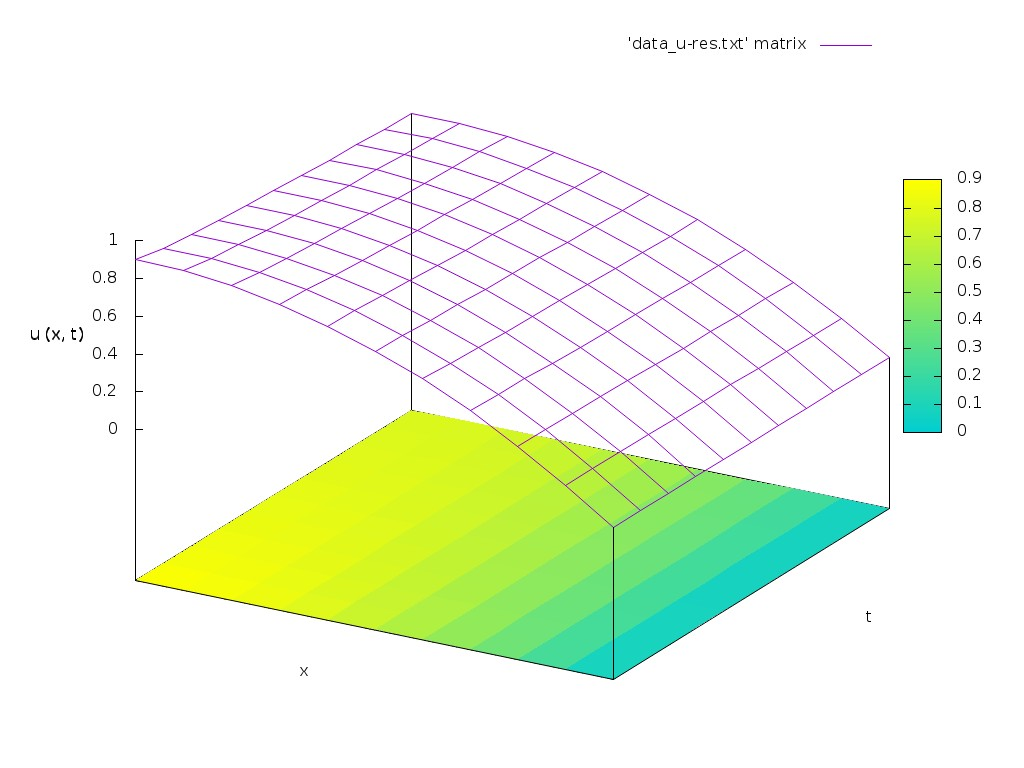
\includegraphics[width=1\linewidth]{../u-res/lines10x10.jpg}} $N=10; M=10$ \\
\end{minipage}
\hfill
\begin{minipage}[h]{0.43\linewidth}
\center{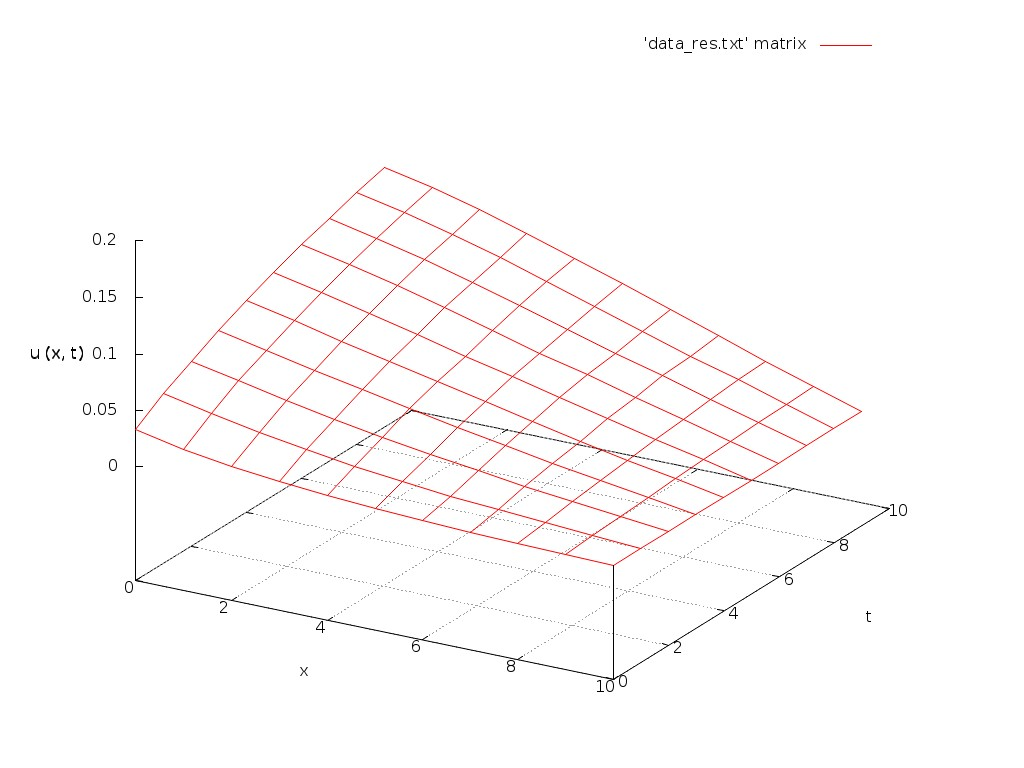
\includegraphics[width=1\linewidth]{../res/lines10x10.jpg}} \textit{Невязка} \\
\end{minipage}
\end{figure}

\begin{figure}[H]
\begin{minipage}[h]{0.43\linewidth}
\center{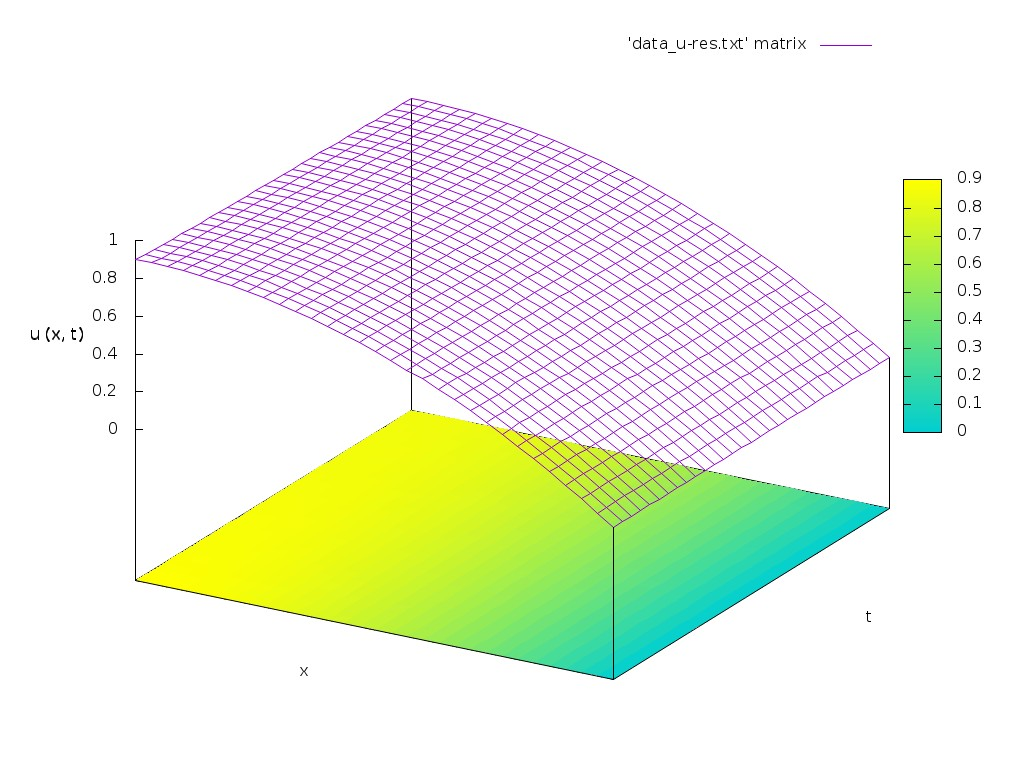
\includegraphics[width=1\linewidth]{../u-res/lines30x30.jpg}} $N=30; M=30$ \\
\end{minipage}
\hfill
\begin{minipage}[h]{0.43\linewidth}
\center{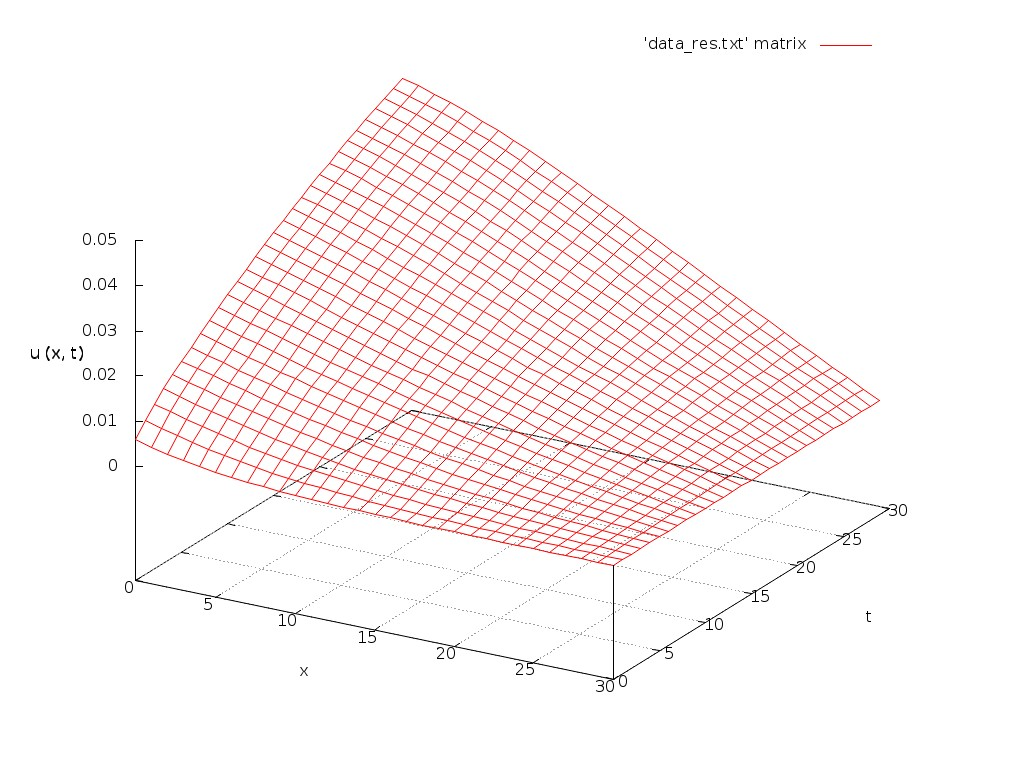
\includegraphics[width=1\linewidth]{../res/lines30x30.jpg}} \textit{Невязка} \\
\end{minipage}
\end{figure}

\begin{figure}[H]
\begin{minipage}[h]{0.43\linewidth}
\center{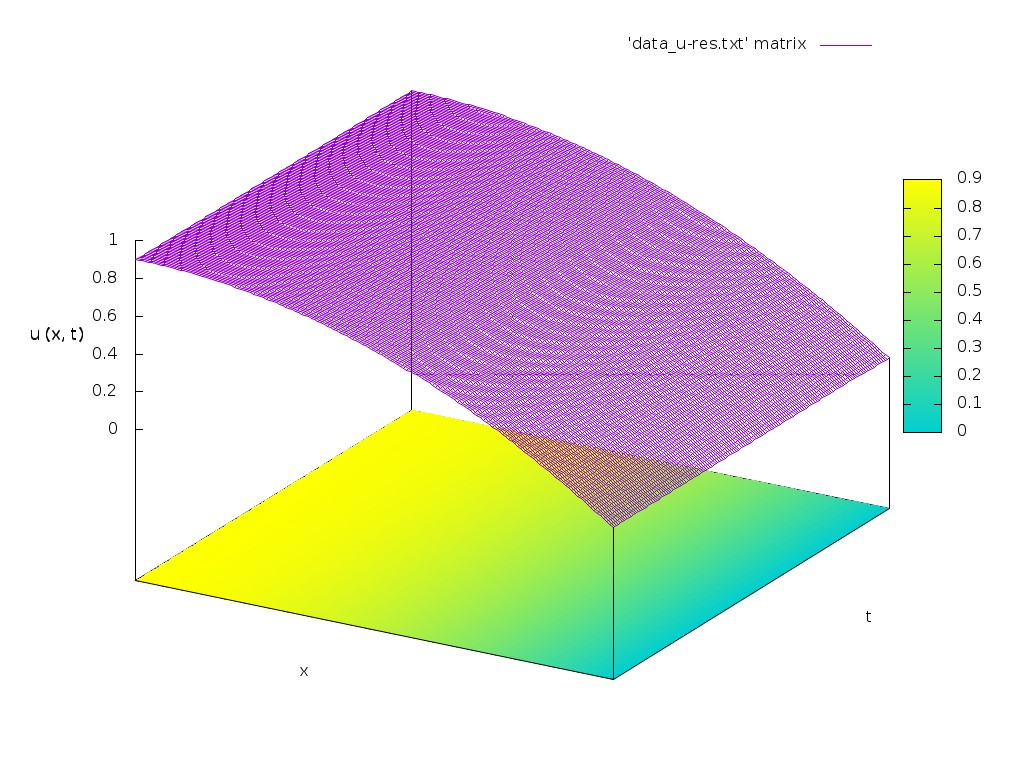
\includegraphics[width=1\linewidth]{../u-res/lines150x150.jpg}} $N=150; M=150$ \\
\end{minipage}
\hfill
\begin{minipage}[h]{0.43\linewidth}
\center{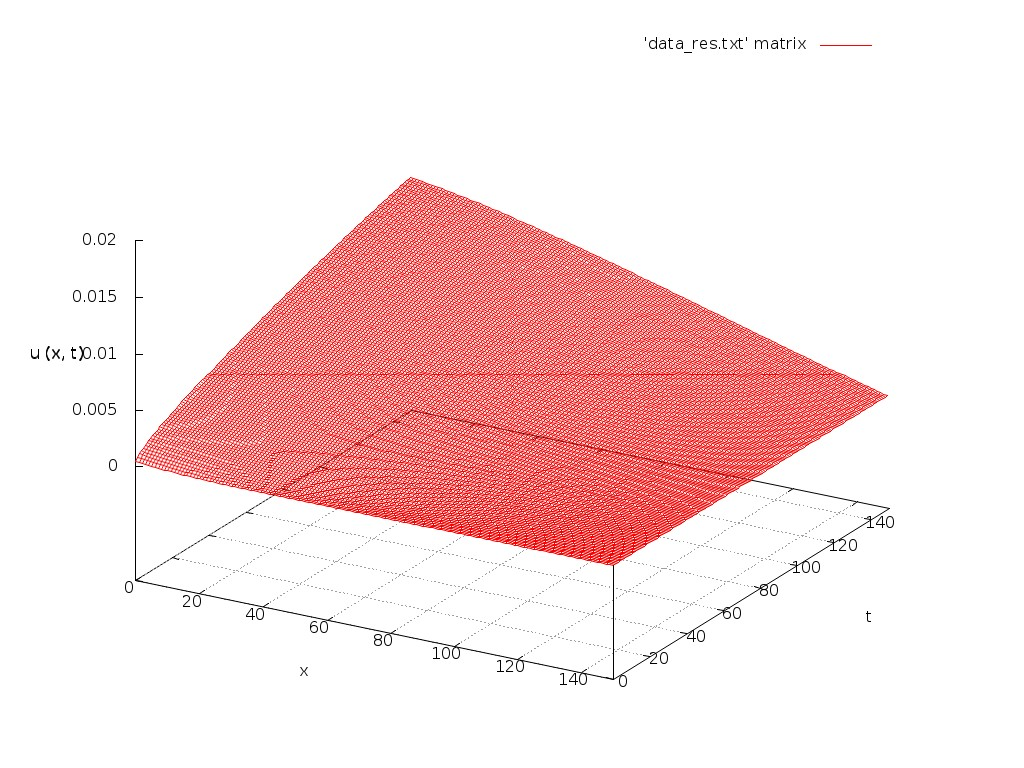
\includegraphics[width=1\linewidth]{../res/lines150x150.jpg}} \textit{Невязка} \\
\end{minipage}
\end{figure}


\section{Графики для $f=u^3$} 
\begin{figure}[H]
\begin{minipage}[h]{0.43\linewidth}
\center{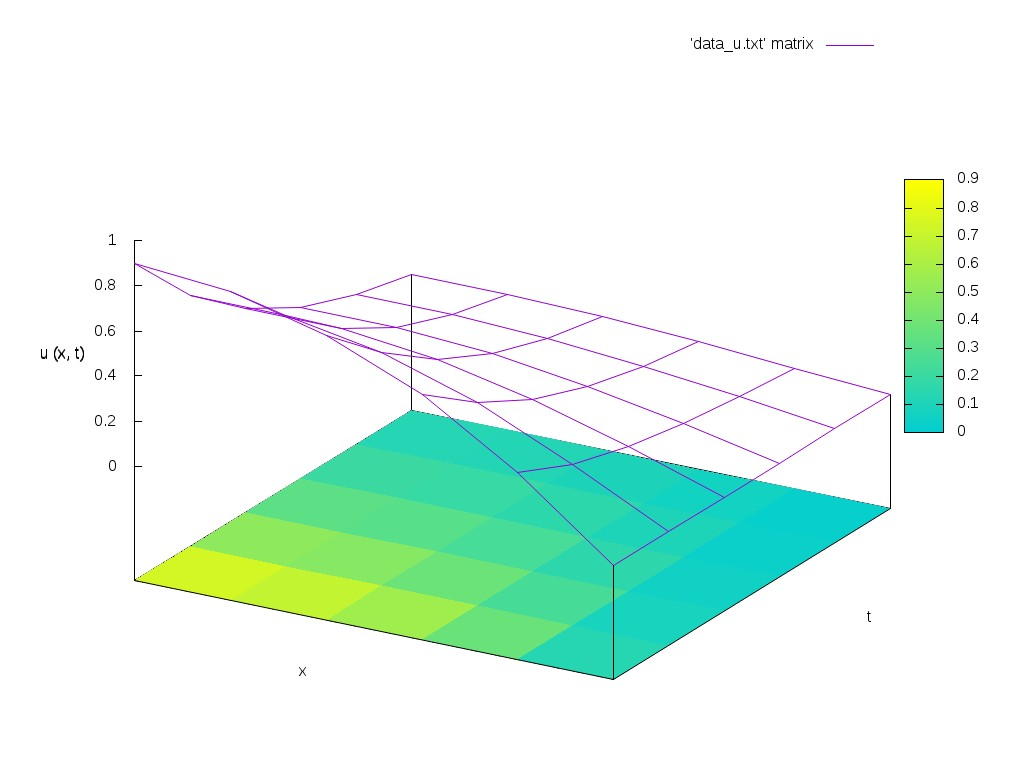
\includegraphics[width=1\linewidth]{../u/lines5x5.jpg}} $N=5; M=5$ \\
\end{minipage}
\hfill
\begin{minipage}[h]{0.43\linewidth}
\center{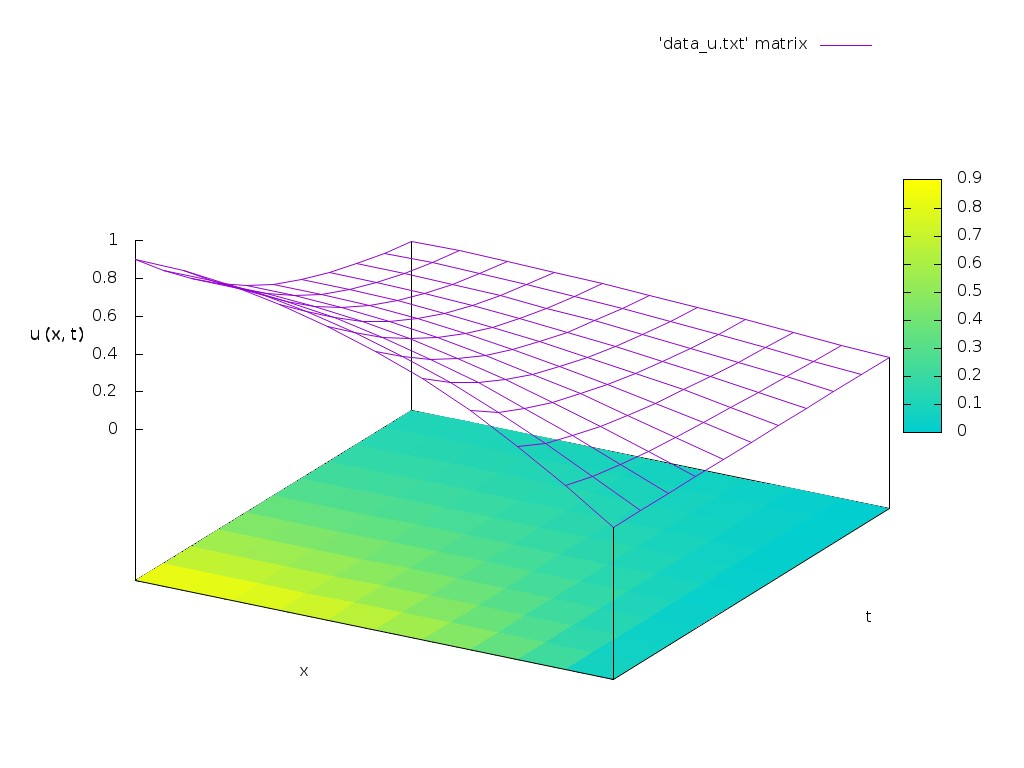
\includegraphics[width=1\linewidth]{../u/lines10x10.jpg}} $N=10; M=10$ \\
\end{minipage}
\end{figure}

\begin{figure}[H]
\begin{minipage}[h]{0.43\linewidth}
\center{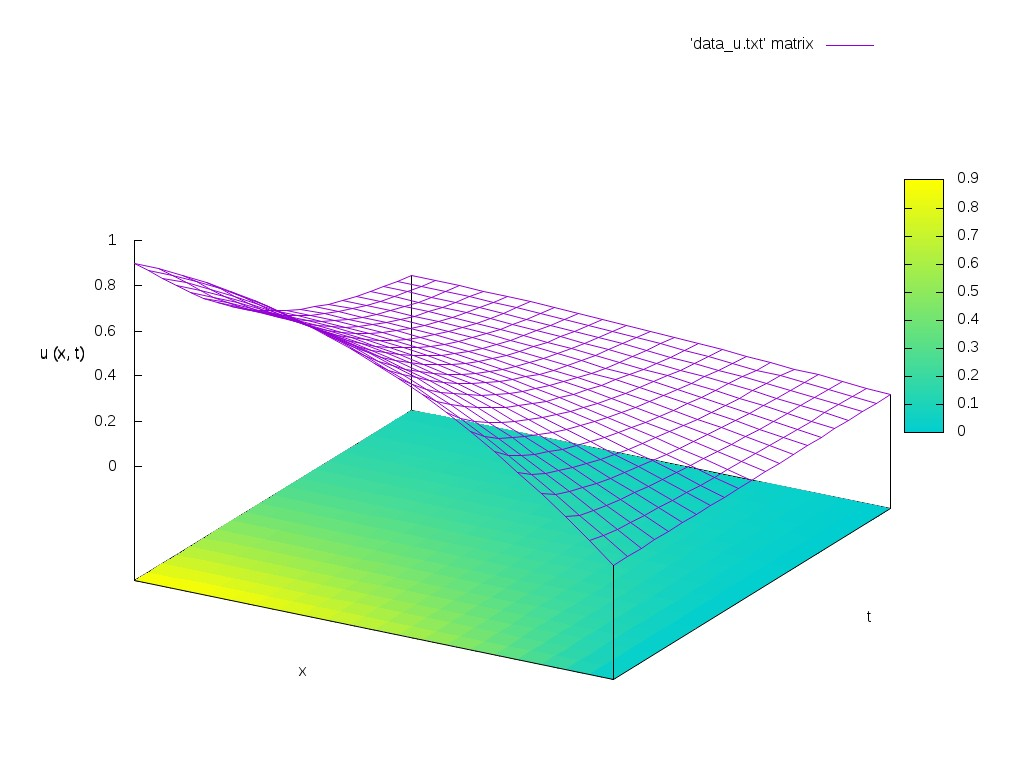
\includegraphics[width=1\linewidth]{../u/lines20x20.jpg}} $N=20; M=20$ \\
\end{minipage}
\hfill
\begin{minipage}[h]{0.43\linewidth}
\center{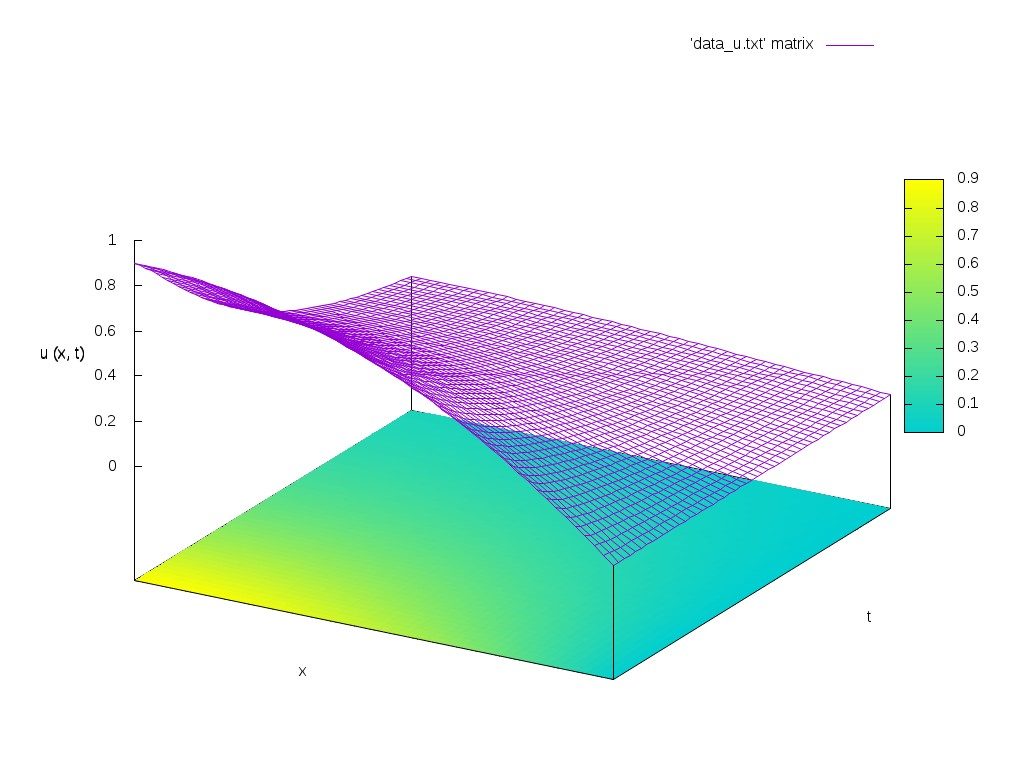
\includegraphics[width=1\linewidth]{../u/lines50x50.jpg}} $N=50; M=50$ \\
\end{minipage}
\end{figure}

\begin{figure}[H]
\begin{minipage}[h]{0.43\linewidth}
\center{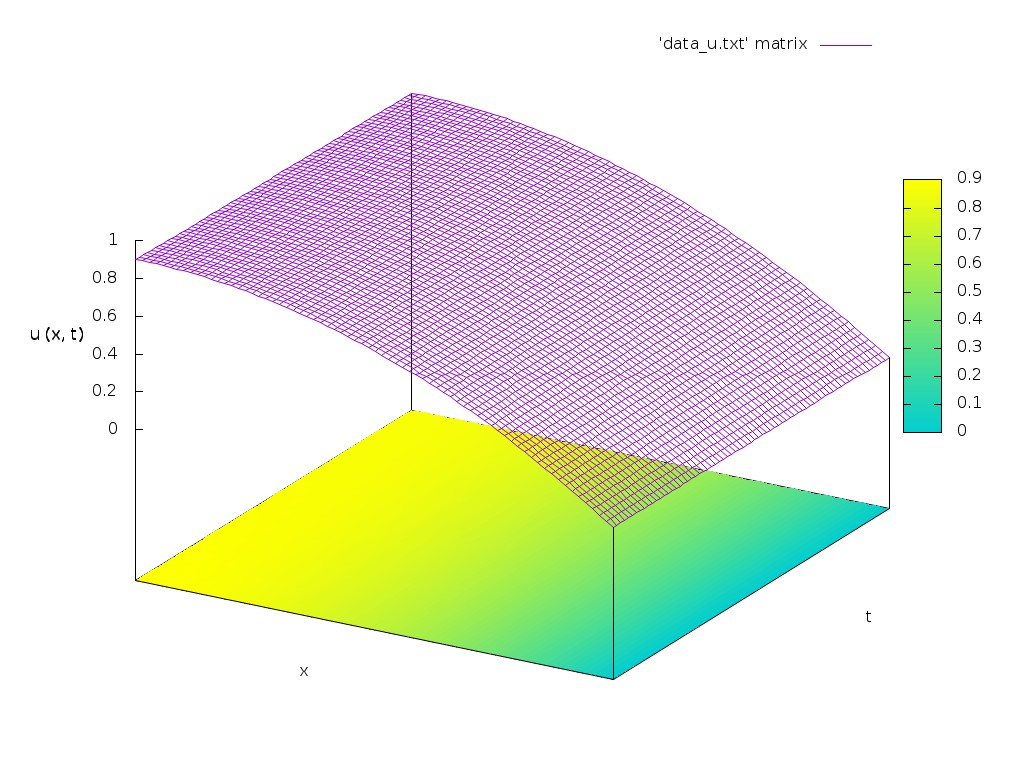
\includegraphics[width=1\linewidth]{../u/lines70x70.jpg}} $N=70; M=70$ \\
\end{minipage}
\hfill
\begin{minipage}[h]{0.43\linewidth}
\center{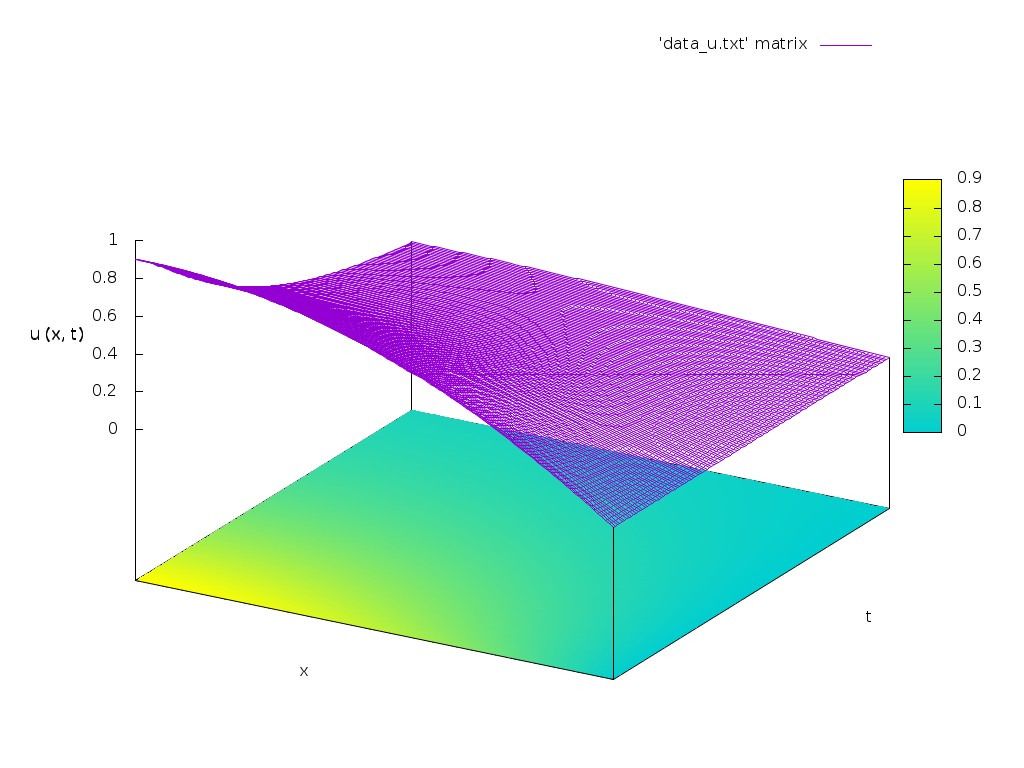
\includegraphics[width=1\linewidth]{../u/lines120x120.jpg}} $N=100; M=100$ \\
\end{minipage}
\end{figure}


\section{Графики для $f=u^3 - \cos \frac{\pi x}{2}$} 
\begin{figure}[H]
\begin{minipage}[h]{0.43\linewidth}
\center{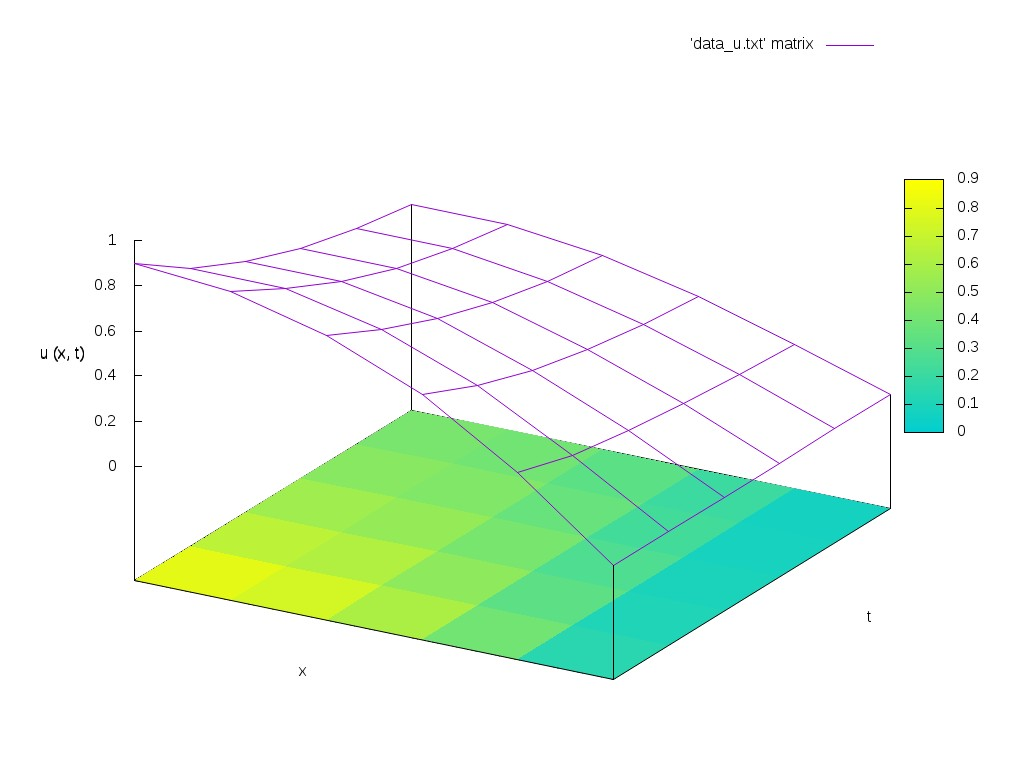
\includegraphics[width=1\linewidth]{../u-cos/lines5x5.jpg}} $N=5; M=5$ \\
\end{minipage}
\hfill
\begin{minipage}[h]{0.43\linewidth}
\center{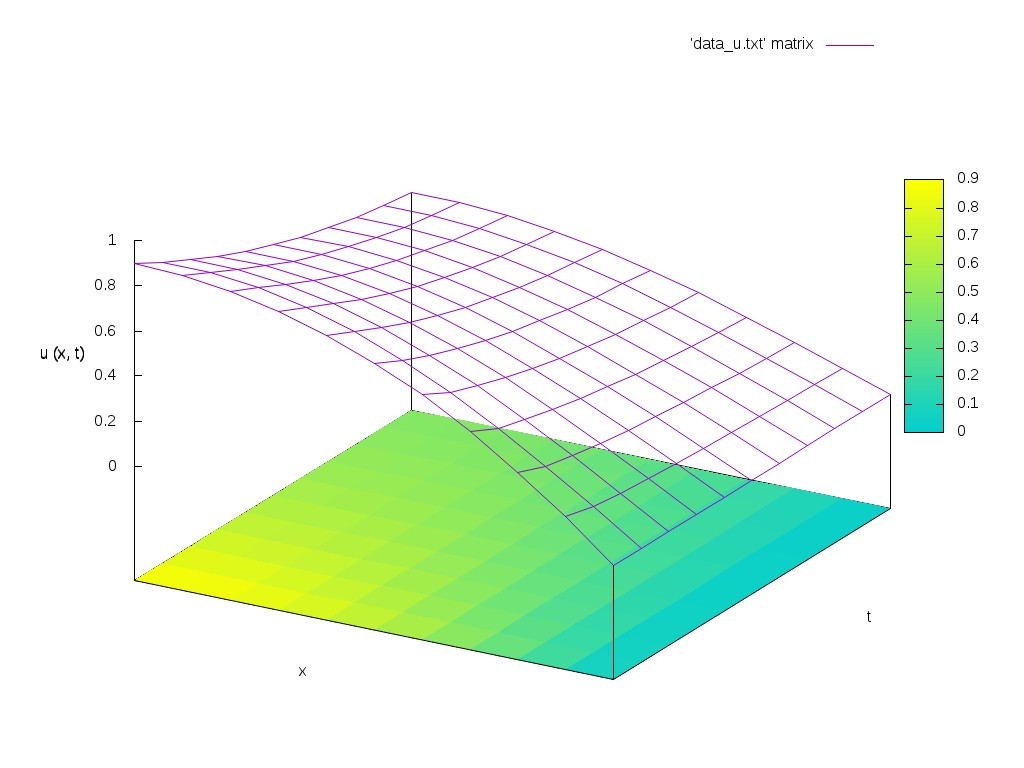
\includegraphics[width=1\linewidth]{../u-cos/lines10x10.jpg}} $N=10; M=10$ \\
\end{minipage}
\end{figure}

\begin{figure}[H]
\begin{minipage}[h]{0.43\linewidth}
\center{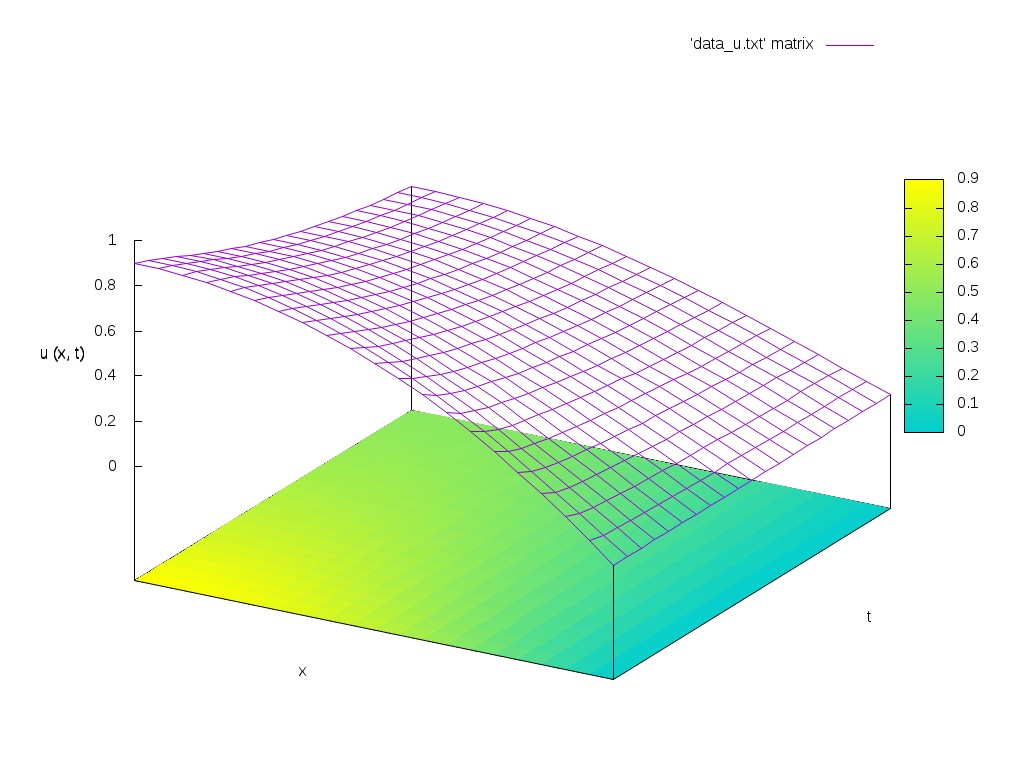
\includegraphics[width=1\linewidth]{../u-cos/lines20x20.jpg}} $N=20; M=20$ \\
\end{minipage}
\hfill
\begin{minipage}[h]{0.43\linewidth}
\center{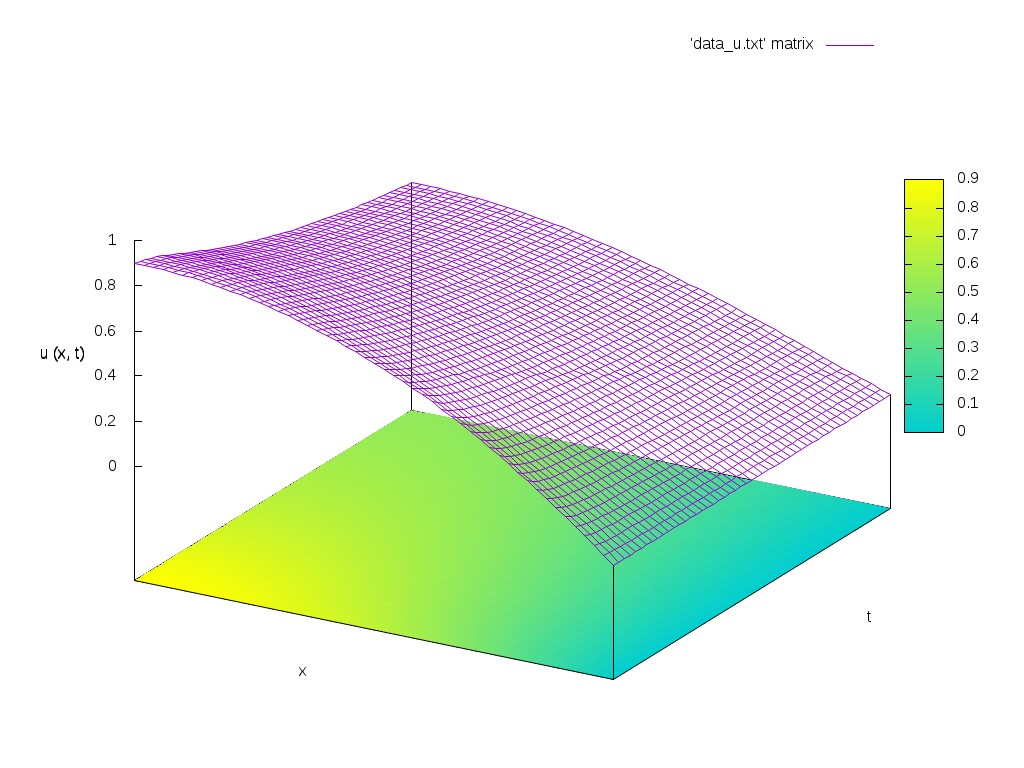
\includegraphics[width=1\linewidth]{../u-cos/lines50x50.jpg}} $N=50; M=50$ \\
\end{minipage}
\end{figure}

\begin{figure}[H]
\begin{minipage}[h]{0.43\linewidth}
\center{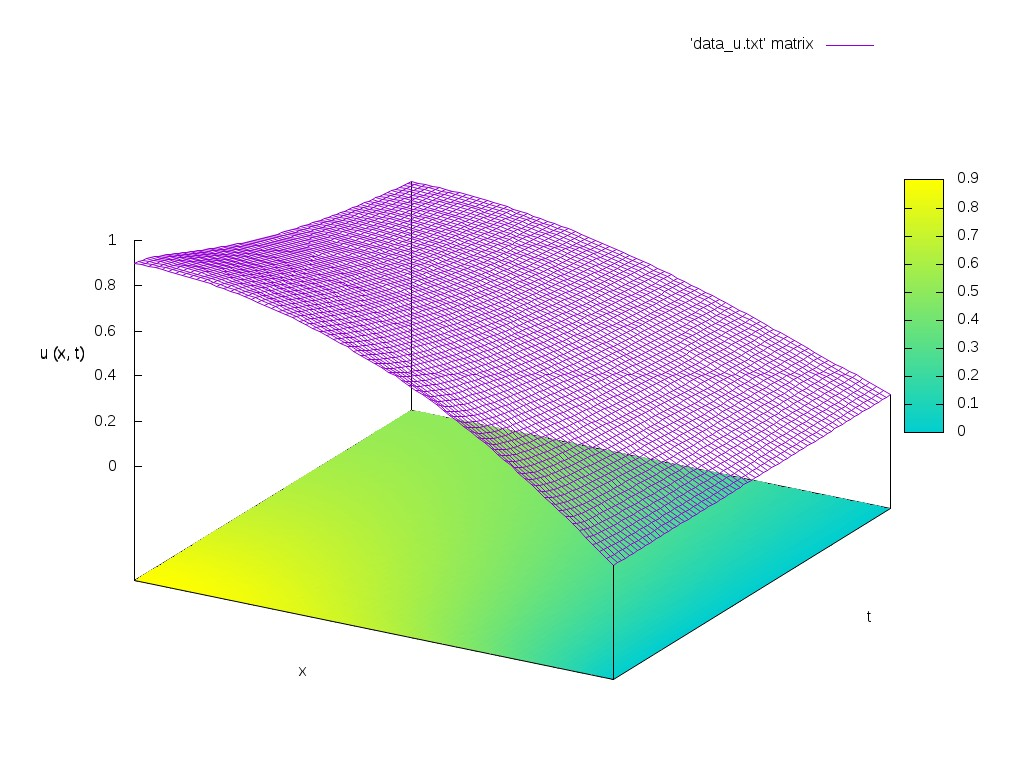
\includegraphics[width=1\linewidth]{../u-cos/lines70x70.jpg}} $N=70; M=70$ \\
\end{minipage}
\hfill
\begin{minipage}[h]{0.43\linewidth}
\center{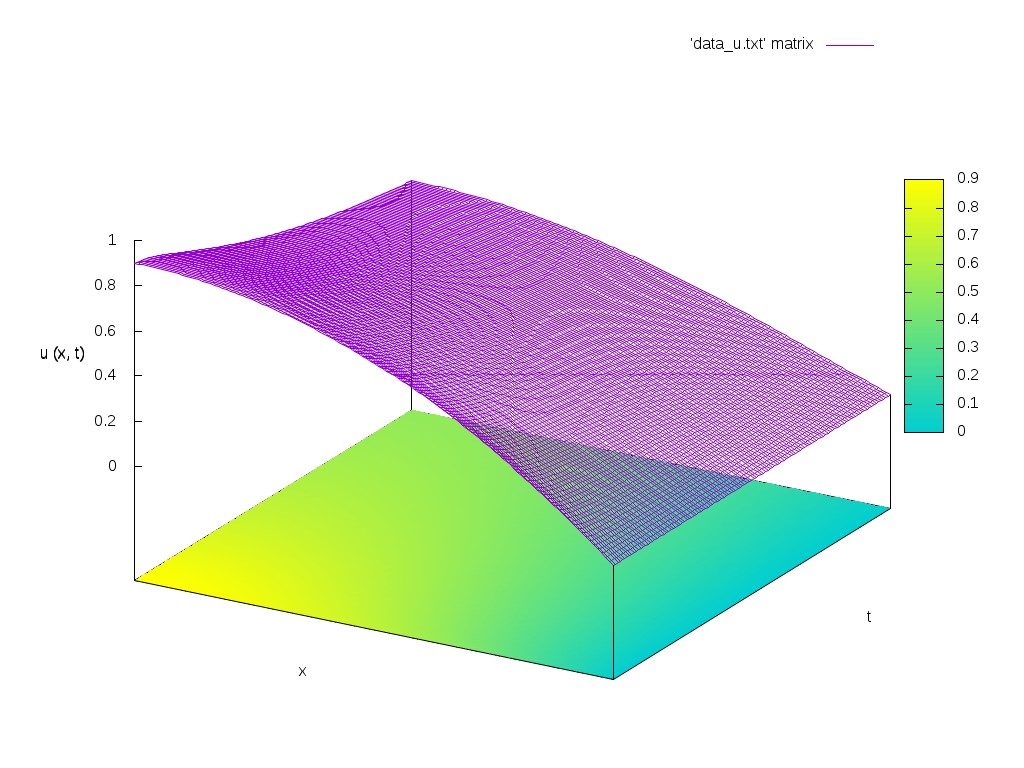
\includegraphics[width=1\linewidth]{../u-cos/lines120x120.jpg}} $N=100; M=100$ \\
\end{minipage}
\end{figure}

\section{Графики для явной схемы для $f=u^3$}
\begin{figure}[H]
\begin{minipage}[h]{0.43\linewidth}
\center{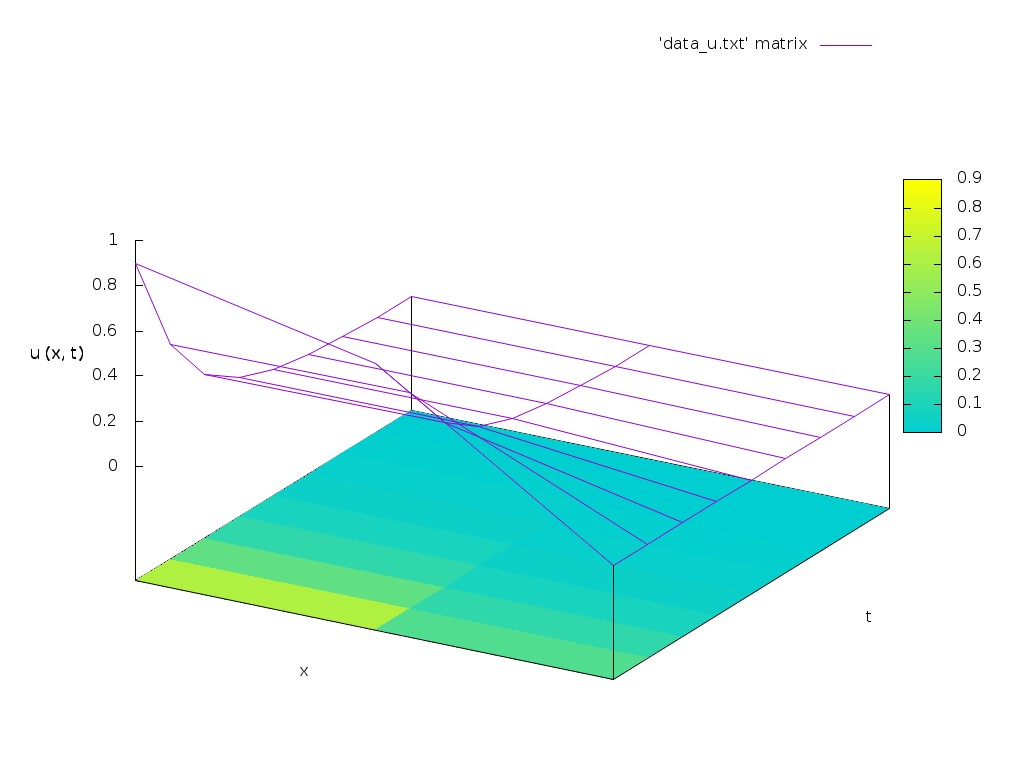
\includegraphics[width=1\linewidth]{../u/non-stab/lines2x8.jpg}} $N=8; M=2;$\\$\cfrac{\tau}{h^2} = \cfrac{1}{2}$ \\
\end{minipage}
\hfill
\begin{minipage}[h]{0.43\linewidth}
\center{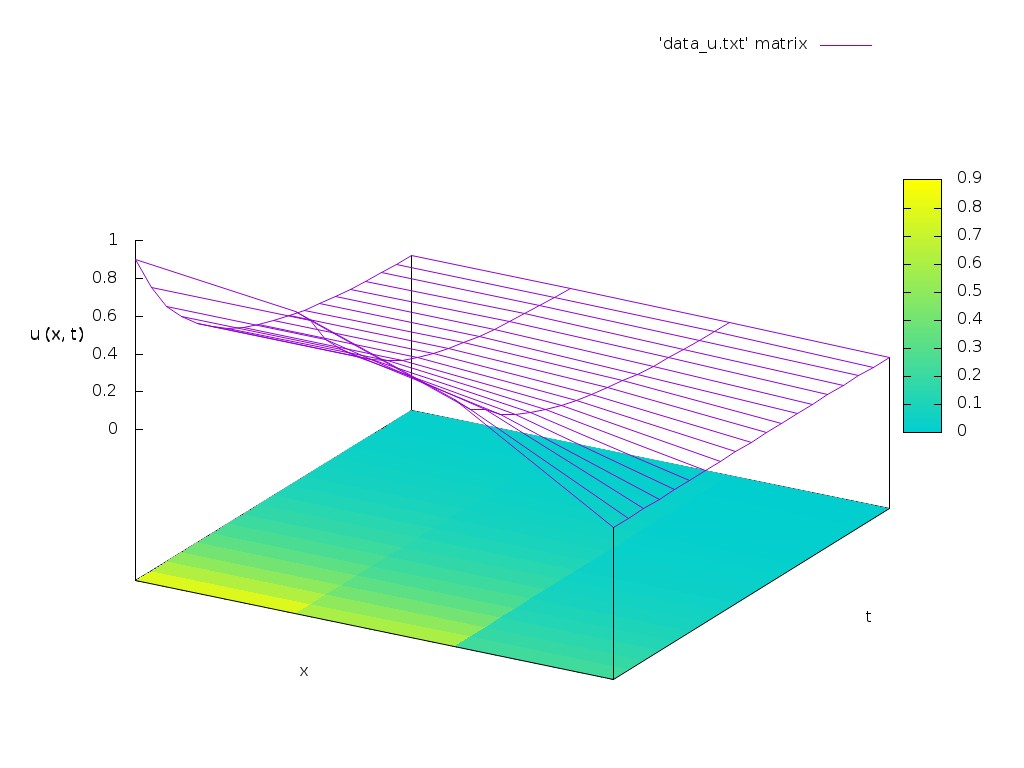
\includegraphics[width=1\linewidth]{../u/non-stab/lines3x18.jpg}} $N=18; M=3;$\\$ \cfrac{\tau}{h^2} = \cfrac{1}{2}$
\end{minipage}

\end{figure}\begin{figure}[H]
\begin{minipage}[h]{0.43\linewidth}
\center{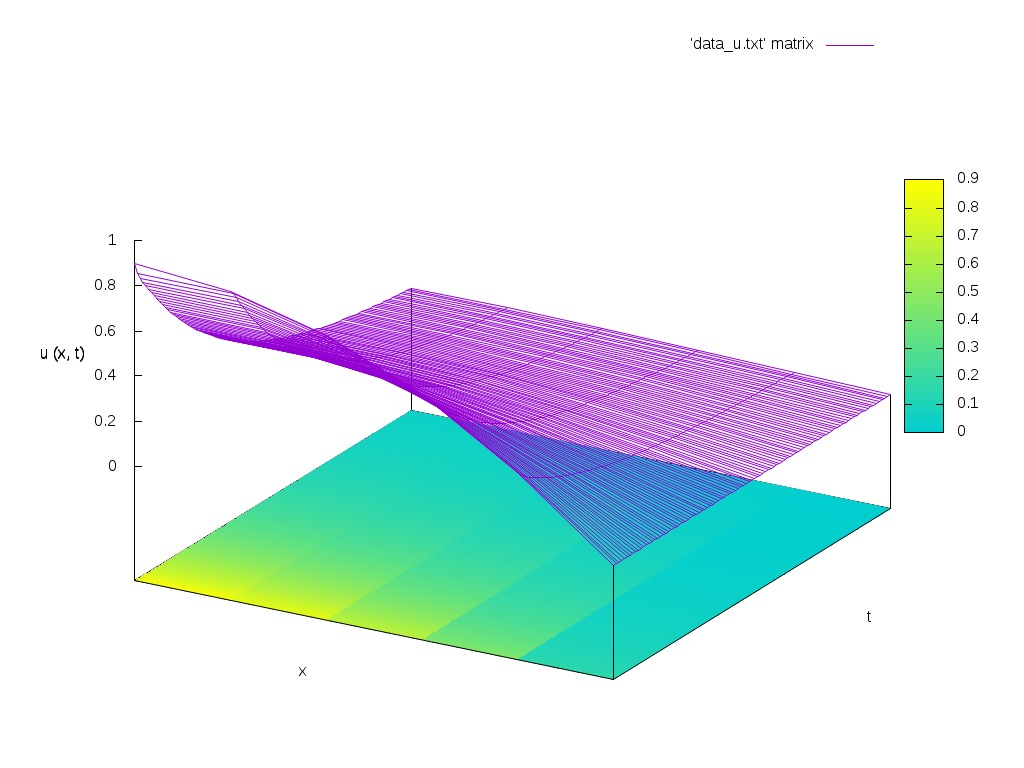
\includegraphics[width=1\linewidth]{../u/non-stab/lines5x100.jpg}} $N=100; M=5;$\\$\cfrac{\tau}{h^2} = \cfrac{1}{4} < \cfrac{1}{2}$ \\
\end{minipage}
\hfill
\begin{minipage}[h]{0.43\linewidth}
\center{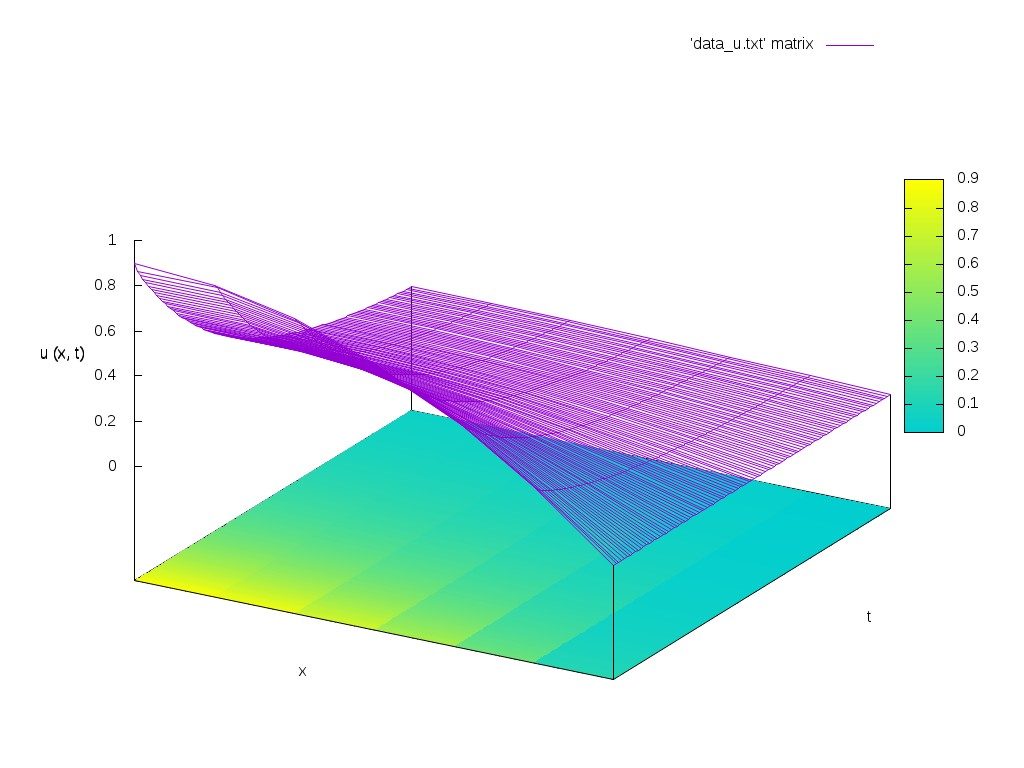
\includegraphics[width=1\linewidth]{../u/non-stab/lines6x100.jpg}} $N=100; M=6;$\\$ \cfrac{\tau}{h^2} = \cfrac{9}{25} < \cfrac{1}{2}$
\end{minipage}
\end{figure}

\begin{figure}[H]
\begin{minipage}[h]{0.43\linewidth}
\center{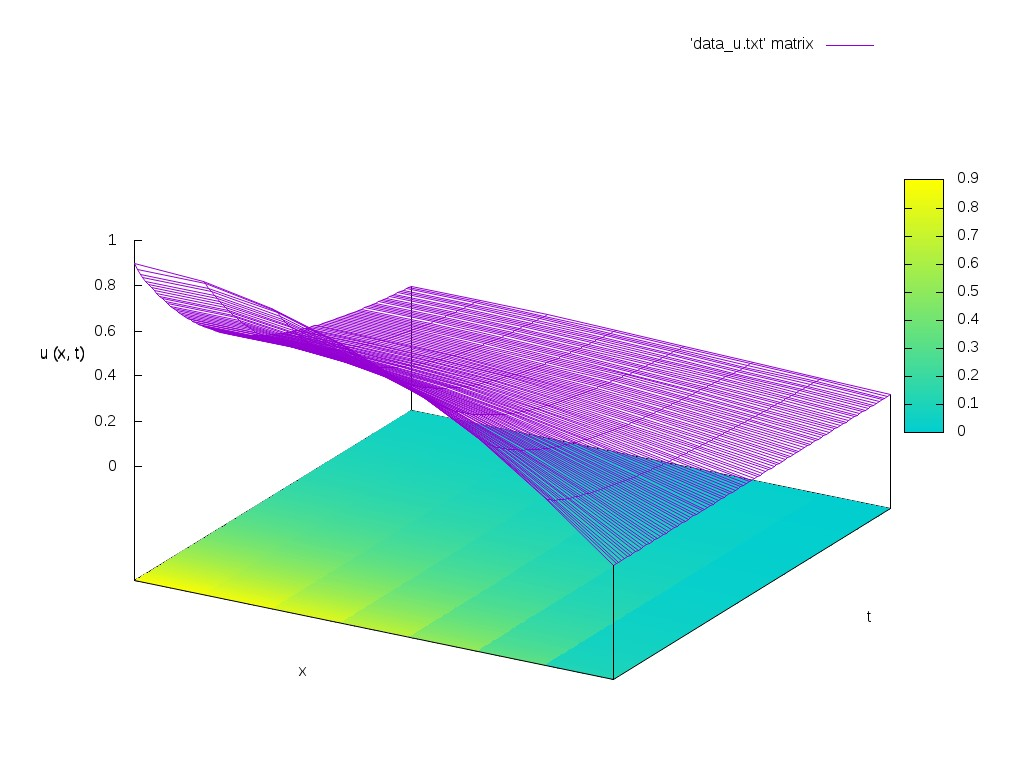
\includegraphics[width=1\linewidth]{../u/non-stab/lines7x100.jpg}} $N=100; M=7;$\\$\cfrac{\tau}{h^2} = \cfrac{49}{100} < \cfrac{1}{2}$ \\
\end{minipage}
\hfill
\begin{minipage}[h]{0.43\linewidth}
\center{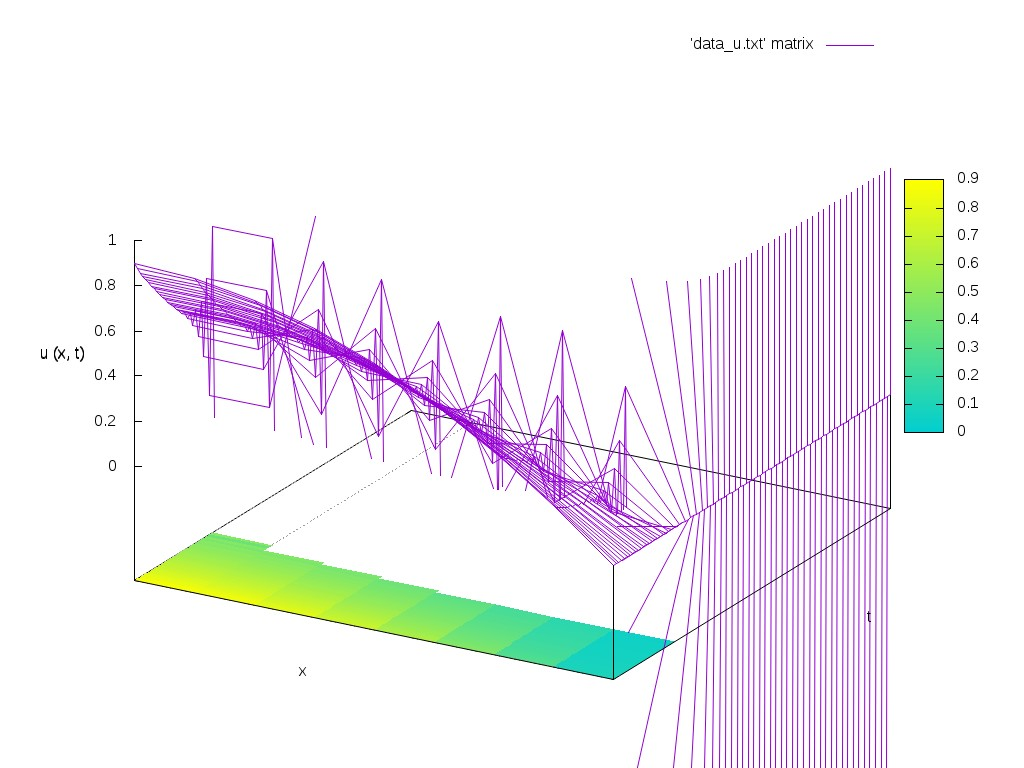
\includegraphics[width=1\linewidth]{../u/non-stab/lines8x100.jpg}} $N=100; M=8;$\\$ \cfrac{\tau}{h^2} = \cfrac{16}{25} > \cfrac{1}{2}$ -- неустойчива
\end{minipage}
\end{figure}

\begin{figure}[H]
\begin{minipage}[h]{0.43\linewidth}
\center{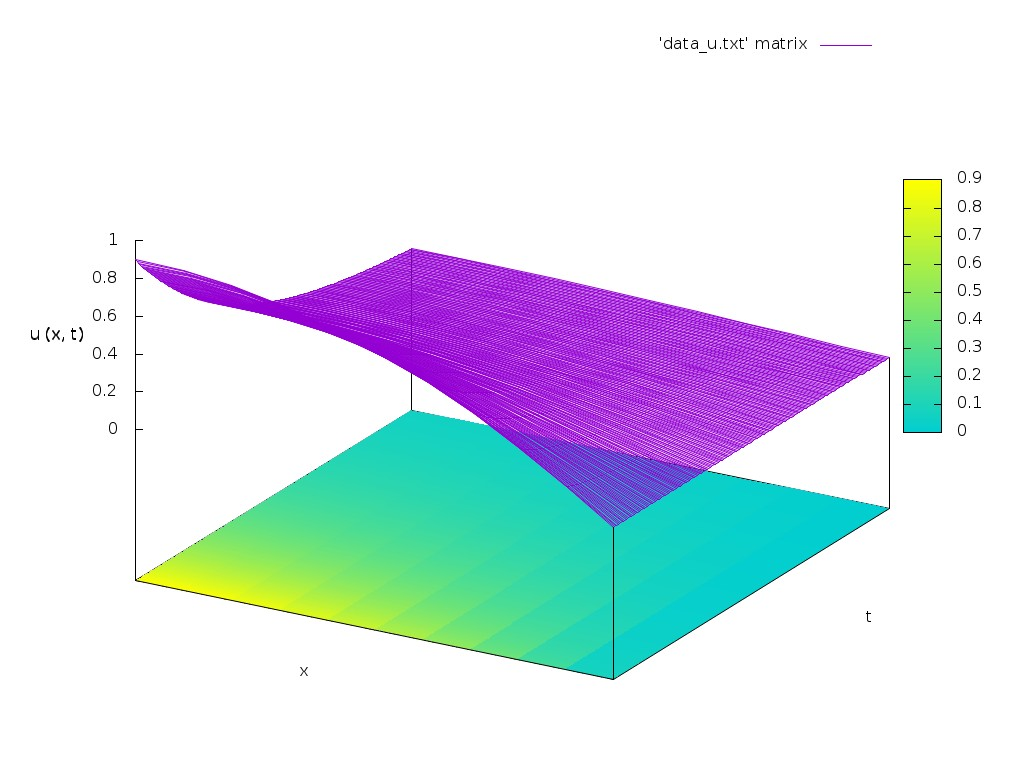
\includegraphics[width=1\linewidth]{../u/non-stab/lines10x210.jpg}} $N=210; M=10;$\\$ \cfrac{\tau}{h^2} > \cfrac{1}{2}$
\end{minipage}
\hfill
\begin{minipage}[h]{0.43\linewidth}
\center{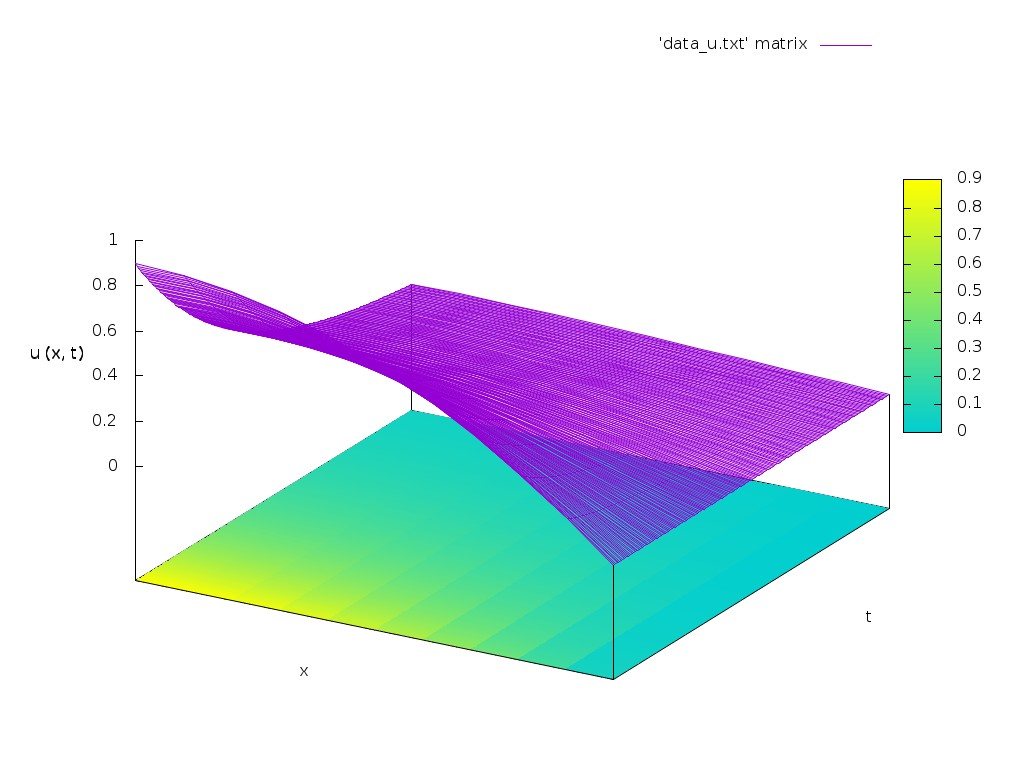
\includegraphics[width=1\linewidth]{../u/non-stab/lines10x200.jpg}} $N=200; M=10;$\\$ \cfrac{\tau}{h^2} = \cfrac{1}{2}$
\end{minipage}
\end{figure}

\begin{figure}[H]
\begin{minipage}[h]{0.43\linewidth}
\center{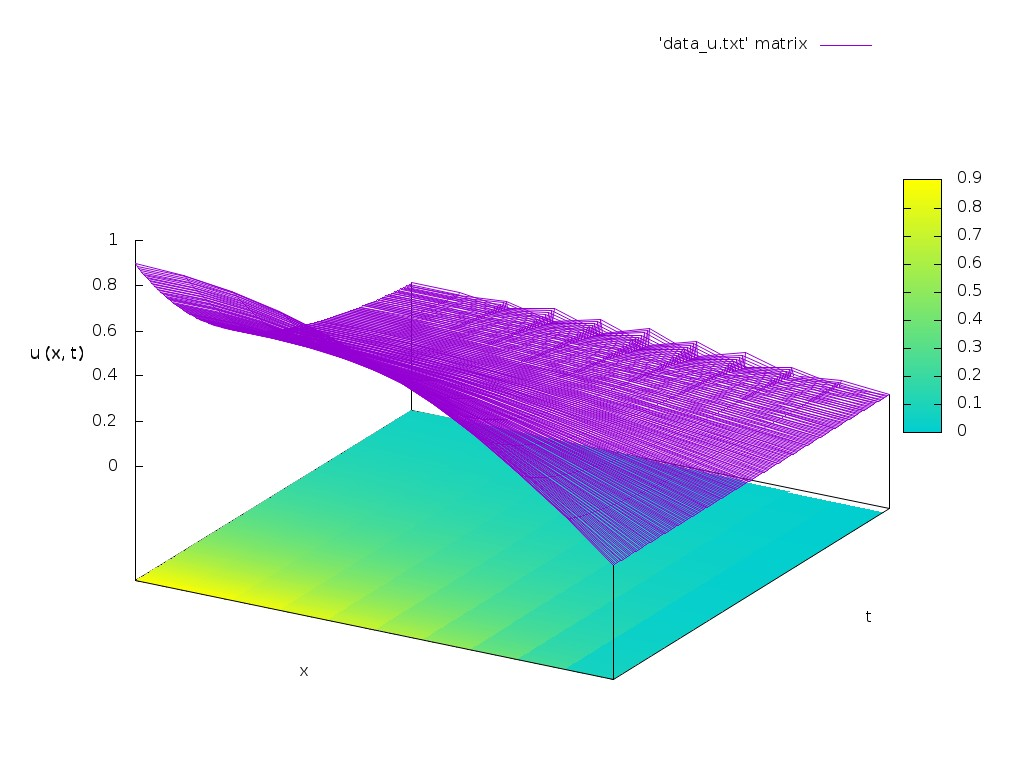
\includegraphics[width=1\linewidth]{../u/non-stab/lines10x190.jpg}} $N=190; M=10;$\\$ \cfrac{\tau}{h^2} = \cfrac{10}{19} > \cfrac{1}{2}$ -- неустойчива
\end{minipage}
\hfill
\begin{minipage}[h]{0.43\linewidth}
\center{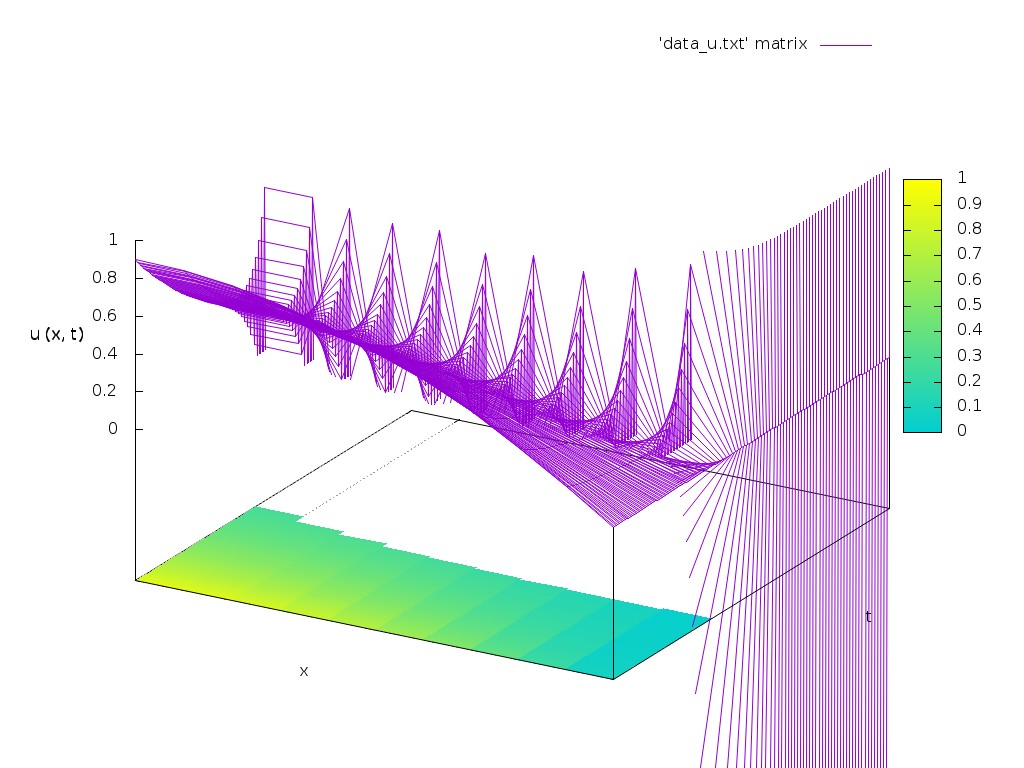
\includegraphics[width=1\linewidth]{../u/non-stab/lines10x180.jpg}} $N=180; M=10;$\\$ \cfrac{\tau}{h^2} = \cfrac{10}{18} > \cfrac{1}{2}$ -- неустойчива
\end{minipage}
\end{figure}

\end{document}